\section{Data acquisition} \label{sec:dataAq}
For a myoelectric prosthetic control system to be able to recognize hand movements it needs to be given prior information on how the movements looks like represented as a EMG-signal - this is also called training the control system. Thus, EMG data needs to be acquired from the user and used to train the control system. The following section describes which types of EMG acquisition techniques that are commonly used.

As presented earlier in \secref{sec:EMG} the source of the EMG signal is motor unit action potentials. The energy generated in action potentials is of a very small size and is measured in microvolts. Very sensitive recording equipments is therefore key in doing electromyography. It is essential to consider the type of electrode intended to use. Electrodes come in various different sizes and shapes and are therefore very depended on the intended measurement site. Typically electrodes made of silver-impregnated plastic are used. They present desired characteristics by being disposable, relatively low price and by having low impedance with the skin. Most electrodes are covered with an adhesive compound in order for them to stick to the skin. These can either be 'dry' or covered with different types of gel, in order to reduce impedance and thereby noise, getting a more accurate EMG recording. Dry electrodes do not use gel, but instead rely on the skin to sweat and thereby decreasing the skin impedance. Dry electrodes should prove better to patients with sensitive skin. Different skin conditions may also effect the electrode-skin impedance. Make-up, scale or much hair increase the impedance, thus the recording site should be prepared by removing hair or cleaning the skin with alcohol wipes. \cite{Cram2012} The following section will introduce the choice of acquisition device used in this project.

\subsection{Myo armband} \label{sub:MYB}
In this project the Myo armband (MYB) from Thalmic Labs will be used for EMG data acquisition. MYB is an electrode armband with eight dry stainless steel electrode-pairs around the inside of the armband, as depicted in \figref{fig:myoarmband}. The advantage of dry electrodes is that they do not need to be disposed after usage as conventional gelled EMG-electrodes \cite{Cram2012}. In addition, MYB can communicate wireless to a computer via Bluetooth 4.0 \cite{Myoarmband2013}. Thus, it is an easy and non-time-consuming device to use both during pilot-testing and for the final experiment. In the following section more information about the MYB will be presented.

MYB records EMG data in a unitless 8-bit resolution. As usual when recording EMG the higher the performed contraction is, the higher the values in the output will be. To avoid interference from power lines a 50 Hz notch filter is built-in in the MYB from the manufacturer. However, the MYB is not able to make any further filtering, therefore this will be implemented later during signal processing described further in \subref{sub:prePros}. The MYB has a 200 Hz sample rate, and thus samples with a lower resolution than the EMG spectrum consists of, which is between 10-500 Hz \cite{Cram2012}. Using MYB will likely result in an aliased EMG signal and confinement in using features representing the frequency information the signal. In \subref{sub:featExtr}, different techniques to counter the negative effect of low-resolution EMG will be proposed for the implementation. 
Besides the EMG sensors the MYB can provide position and orientation information, using its three inertial measurement units consisting of a three axis gyroscope, a three axis magnetometer and a three axis accelerometer. This inertial information is sampled at 50 Hz. \cite{Myoarmband2013} \\
When initiating the wearing of the armband there is two calibration phases the user must follow before the armband is ready to use - the warm-up phase and the sync phase. During the warm-up phase the armband is ensuring as strong electrical connection with the muscles in the forearm as possible. This is mainly provided by light sweating on the skin under the electrodes, which improve the connection similar to electrode gel \cite{Cram2012}. During the sync phase, the armband determines its orientation in space, position and on which arm it is placed. The MYB works most optimal when fitted tightly on the thickest part of the forearm. For users with smaller forearms a set of clips can be added for the armband to get a constrained grip. \cite{Myoarmband2013}

\begin{figure}[H]                 
	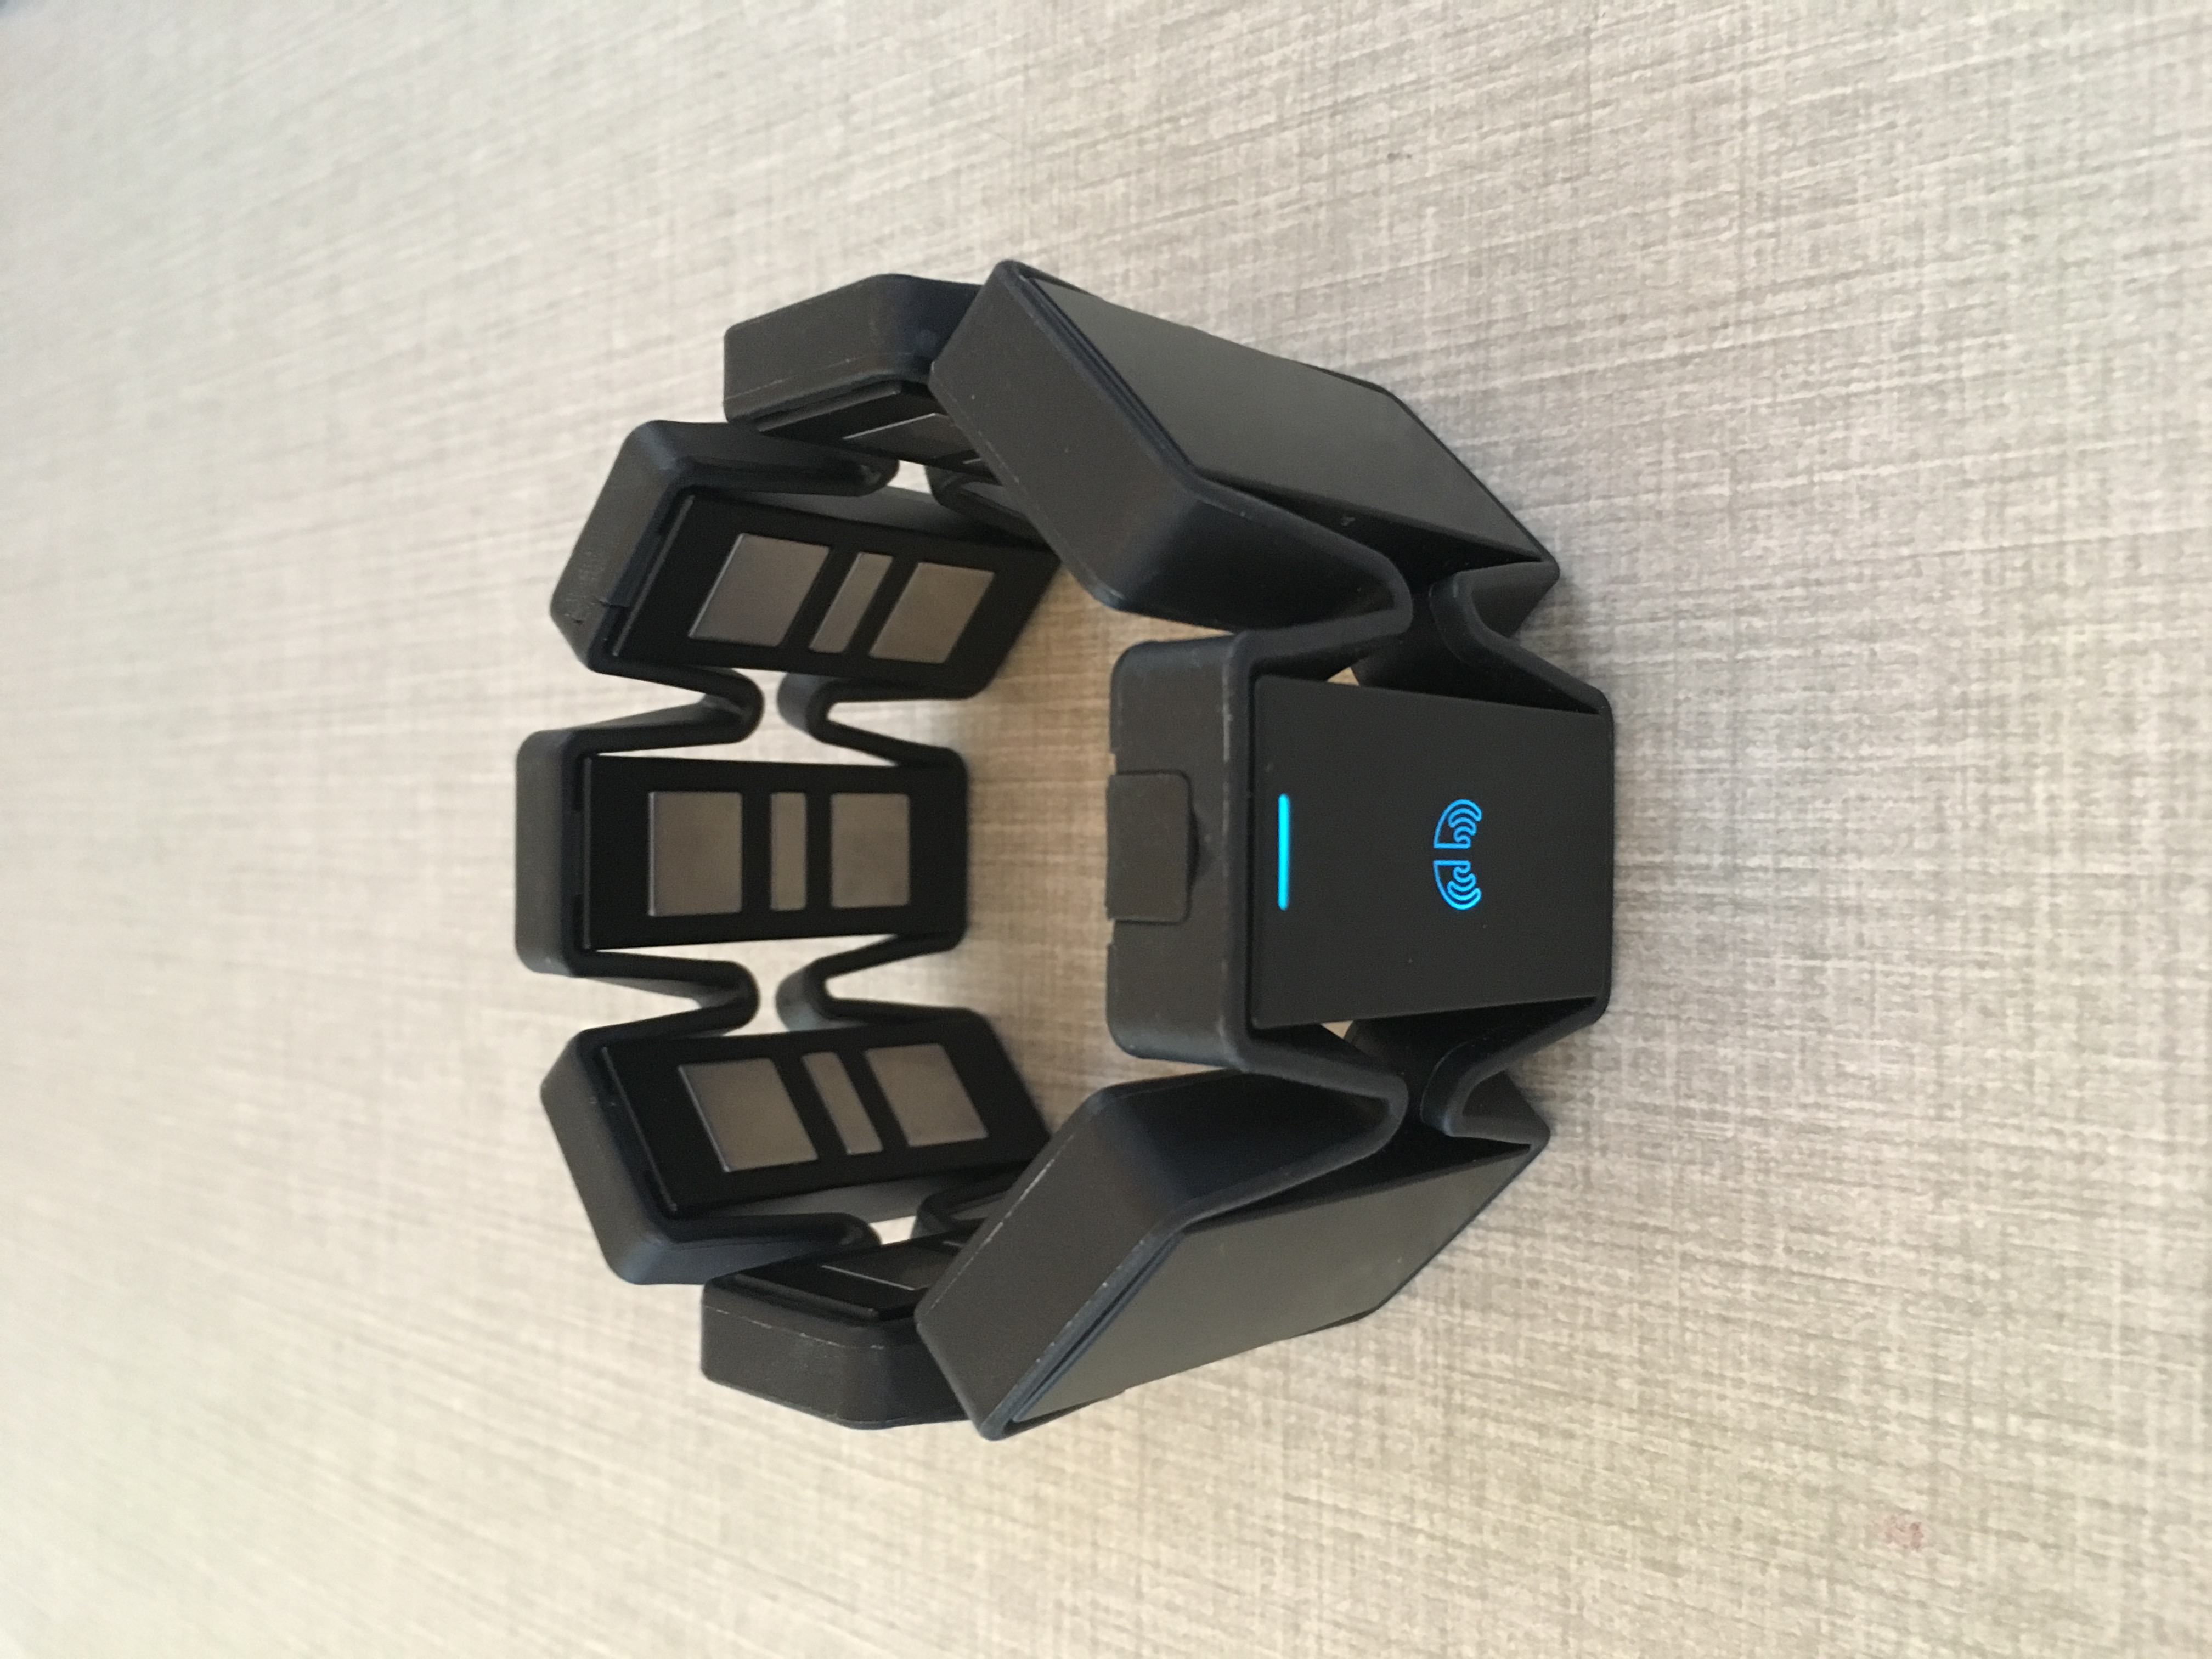
\includegraphics[width=.4\textwidth]{figures/xBackground/myoband}  
	\caption{MYB from Thalmic Labs. The number on each channel indicates which channel corresponds to which column in the digital output, when acquiring data from MYB.}
	\label{fig:myoarmband} 
\end{figure}